\documentclass[]{article}
\usepackage{lmodern}
\usepackage{amssymb,amsmath}
\usepackage{ifxetex,ifluatex}
\usepackage{fixltx2e} % provides \textsubscript
\ifnum 0\ifxetex 1\fi\ifluatex 1\fi=0 % if pdftex
  \usepackage[T1]{fontenc}
  \usepackage[utf8]{inputenc}
\else % if luatex or xelatex
  \ifxetex
    \usepackage{mathspec}
  \else
    \usepackage{fontspec}
  \fi
  \defaultfontfeatures{Ligatures=TeX,Scale=MatchLowercase}
\fi
% use upquote if available, for straight quotes in verbatim environments
\IfFileExists{upquote.sty}{\usepackage{upquote}}{}
% use microtype if available
\IfFileExists{microtype.sty}{%
\usepackage{microtype}
\UseMicrotypeSet[protrusion]{basicmath} % disable protrusion for tt fonts
}{}
\usepackage[margin=1in]{geometry}
\usepackage{hyperref}
\hypersetup{unicode=true,
            pdftitle={MT4113 - Report},
            pdfauthor={180024570},
            pdfborder={0 0 0},
            breaklinks=true}
\urlstyle{same}  % don't use monospace font for urls
\usepackage{graphicx,grffile}
\makeatletter
\def\maxwidth{\ifdim\Gin@nat@width>\linewidth\linewidth\else\Gin@nat@width\fi}
\def\maxheight{\ifdim\Gin@nat@height>\textheight\textheight\else\Gin@nat@height\fi}
\makeatother
% Scale images if necessary, so that they will not overflow the page
% margins by default, and it is still possible to overwrite the defaults
% using explicit options in \includegraphics[width, height, ...]{}
\setkeys{Gin}{width=\maxwidth,height=\maxheight,keepaspectratio}
\IfFileExists{parskip.sty}{%
\usepackage{parskip}
}{% else
\setlength{\parindent}{0pt}
\setlength{\parskip}{6pt plus 2pt minus 1pt}
}
\setlength{\emergencystretch}{3em}  % prevent overfull lines
\providecommand{\tightlist}{%
  \setlength{\itemsep}{0pt}\setlength{\parskip}{0pt}}
\setcounter{secnumdepth}{5}
% Redefines (sub)paragraphs to behave more like sections
\ifx\paragraph\undefined\else
\let\oldparagraph\paragraph
\renewcommand{\paragraph}[1]{\oldparagraph{#1}\mbox{}}
\fi
\ifx\subparagraph\undefined\else
\let\oldsubparagraph\subparagraph
\renewcommand{\subparagraph}[1]{\oldsubparagraph{#1}\mbox{}}
\fi

%%% Use protect on footnotes to avoid problems with footnotes in titles
\let\rmarkdownfootnote\footnote%
\def\footnote{\protect\rmarkdownfootnote}

%%% Change title format to be more compact
\usepackage{titling}

% Create subtitle command for use in maketitle
\newcommand{\subtitle}[1]{
  \posttitle{
    \begin{center}\large#1\end{center}
    }
}

\setlength{\droptitle}{-2em}

  \title{MT4113 - Report}
    \pretitle{\vspace{\droptitle}\centering\huge}
  \posttitle{\par}
    \author{180024570}
    \preauthor{\centering\large\emph}
  \postauthor{\par}
      \predate{\centering\large\emph}
  \postdate{\par}
    \date{07/11/2018}

\usepackage{subfig}
\usepackage{booktabs}
\usepackage{longtable}
\usepackage{array}
\usepackage{multirow}
\usepackage[table]{xcolor}
\usepackage{wrapfig}
\usepackage{float}
\usepackage{colortbl}
\usepackage{pdflscape}
\usepackage{tabu}
\usepackage{threeparttable}
\usepackage{threeparttablex}
\usepackage[normalem]{ulem}
\usepackage{makecell}

\usepackage{booktabs} \usepackage{longtable} \usepackage{array} \usepackage{enumitem} \usepackage{multirow} \usepackage[table]{xcolor} \usepackage{wrapfig} \usepackage{float} \floatplacement{figure}{H} \usepackage[bottom]{footmisc}

\begin{document}
\maketitle

\emph{I confirm that the following report and associated code is my own
work, except where clearly indicated.}

\newpage

\section*{\centering Abstract}

More than 17 million people voted to leave the EU in 2016 Referendum in
the UK. This statistical report investigated the difference of approval
rates of Brexit in England and the rest of the UK by carrying out both
parametric and non-parametric tests. Particularly, Monte Carlo
simulation is conducted on the referendum dataset by regions, to
research the properties of those statistical tests under a range of
different scenarios. \emph{add a bit summary of result}

\newpage

\hypertarget{motivation}{%
\section{Motivation}\label{motivation}}

Hundreds of thousands of people marched to London's Parliament Square
for a referendum on the final Brexit deal in late October(BBC News,
2018). In the EU referendum in 2016, approximately 52\%, or more than 17
million people in the UK, voted to leave the European Union (Becker,
Fetzer \& Novy, 2017). To investigate what voters in different nations
of the UK vote for, the dataset of EU referendum results by
regions(Electoral Commission, 2016) are statistically analysed and
tested in this report. The dateset contains numerous variates regarding
the referendum outcome, yet only \emph{Region} and \emph{Percent Leave}
are concerned in terms of our research objectives.

\begin{figure}
\centering
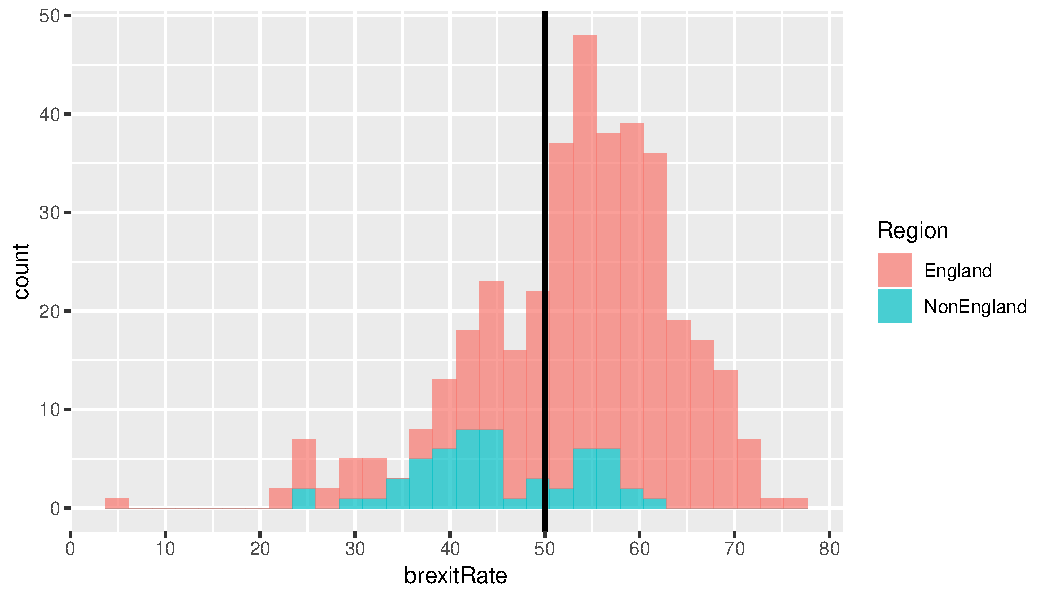
\includegraphics{../figure/datasetHist.pdf}
\caption{Vote Outcome in England and Non-England Regions}
\end{figure}

According to the histogram of leave votes, it seems that England regions
tend to be more supportive of Brexit than other regions. Hence, The
research question is proposed as that

\begin{itemize}
\tightlist
\item
  \emph{Were approval rates of Brexit greater in England or rest of the
  UK in 2016 referendum?}
\end{itemize}

On the basis of our research question, regions are categorized as
England or Non-England, thus, One-tail Student's T test and Mann-Whitney
U test are chosen to be conducted to compare the difference of mean
approval rates of Brexit. Moreover, 1000-iteration Monte Carlo
simulations are carried out under a range of scenarios in order to
investigate power and size of these tests.

\hypertarget{methodology}{%
\section{Methodology}\label{methodology}}

Here to describe methods! Here to describe methods! Here to describe
methods! Here to describe methods! Here to describe methods!

\hypertarget{result-and-discussion}{%
\section{Result and Discussion}\label{result-and-discussion}}

The power of parametric and non-parametric tests, in terms of different
sample sizes and effect sizes, are calculated based on 1000 simulated
datasets, and the result are shown in two tables below.

\begin{table}

\caption{\label{tab:power-tables}Power of Student's T Test}
\centering
\begin{tabular}[t]{lrrrrrrrrrr}
\toprule
\multicolumn{ 1}{c}{\bfseries Sample Size} & \multicolumn{10}{c}{\bfseries Effect Size} \\
\cmidrule(l{2pt}r{2pt}){1-1} \cmidrule(l{2pt}r{2pt}){2-11}
  & 1 & 2 & 3 & 4 & 5 & 6 & 7 & 8 & 9 & 10\\
\midrule
10 & 0.000 & 0.001 & 0.009 & 0.051 & 0.144 & 0.32 & 0.543 & 0.743 & 0.883 & 0.953\\
50 & 0.000 & 0.006 & 0.510 & 0.992 & 1.000 & 1.00 & 1.000 & 1.000 & 1.000 & 1.000\\
100 & 0.000 & 0.323 & 1.000 & 1.000 & 1.000 & 1.00 & 1.000 & 1.000 & 1.000 & 1.000\\
150 & 0.000 & 0.923 & 1.000 & 1.000 & 1.000 & 1.00 & 1.000 & 1.000 & 1.000 & 1.000\\
200 & 0.001 & 1.000 & 1.000 & 1.000 & 1.000 & 1.00 & 1.000 & 1.000 & 1.000 & 1.000\\
\addlinespace
300 & 0.047 & 1.000 & 1.000 & 1.000 & 1.000 & 1.00 & 1.000 & 1.000 & 1.000 & 1.000\\
400 & 0.296 & 1.000 & 1.000 & 1.000 & 1.000 & 1.00 & 1.000 & 1.000 & 1.000 & 1.000\\
500 & 0.720 & 1.000 & 1.000 & 1.000 & 1.000 & 1.00 & 1.000 & 1.000 & 1.000 & 1.000\\
700 & 0.995 & 1.000 & 1.000 & 1.000 & 1.000 & 1.00 & 1.000 & 1.000 & 1.000 & 1.000\\
1000 & 1.000 & 1.000 & 1.000 & 1.000 & 1.000 & 1.00 & 1.000 & 1.000 & 1.000 & 1.000\\
\bottomrule
\end{tabular}
\end{table}

\begin{table}

\caption{\label{tab:power-tables}Power of Mann-Whitney U Test}
\centering
\begin{tabular}[t]{lrrrrrrrrrr}
\toprule
\multicolumn{ 1}{c}{\bfseries Sample Size} & \multicolumn{10}{c}{\bfseries Effect Size} \\
\cmidrule(l{2pt}r{2pt}){1-1} \cmidrule(l{2pt}r{2pt}){2-11}
  & 1 & 2 & 3 & 4 & 5 & 6 & 7 & 8 & 9 & 10\\
\midrule
10 & 0.001 & 0.003 & 0.016 & 0.065 & 0.185 & 0.358 & 0.541 & 0.724 & 0.848 & 0.92\\
50 & 0.000 & 0.031 & 0.565 & 0.982 & 1.000 & 1.000 & 1.000 & 1.000 & 1.000 & 1.00\\
100 & 0.000 & 0.372 & 0.998 & 1.000 & 1.000 & 1.000 & 1.000 & 1.000 & 1.000 & 1.00\\
150 & 0.003 & 0.892 & 1.000 & 1.000 & 1.000 & 1.000 & 1.000 & 1.000 & 1.000 & 1.00\\
200 & 0.009 & 0.997 & 1.000 & 1.000 & 1.000 & 1.000 & 1.000 & 1.000 & 1.000 & 1.00\\
\addlinespace
300 & 0.072 & 1.000 & 1.000 & 1.000 & 1.000 & 1.000 & 1.000 & 1.000 & 1.000 & 1.00\\
400 & 0.305 & 1.000 & 1.000 & 1.000 & 1.000 & 1.000 & 1.000 & 1.000 & 1.000 & 1.00\\
500 & 0.634 & 1.000 & 1.000 & 1.000 & 1.000 & 1.000 & 1.000 & 1.000 & 1.000 & 1.00\\
700 & 0.975 & 1.000 & 1.000 & 1.000 & 1.000 & 1.000 & 1.000 & 1.000 & 1.000 & 1.00\\
1000 & 1.000 & 1.000 & 1.000 & 1.000 & 1.000 & 1.000 & 1.000 & 1.000 & 1.000 & 1.00\\
\bottomrule
\end{tabular}
\end{table}

\begin{figure}
\centering
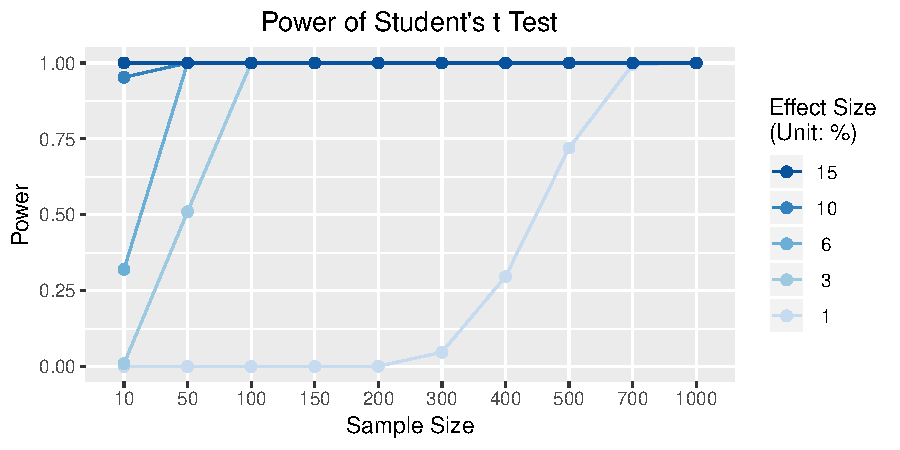
\includegraphics{../figure/power_t.pdf}
\caption{Power of Student's t Test under Different Scenarios}
\end{figure}

\begin{figure}
\centering
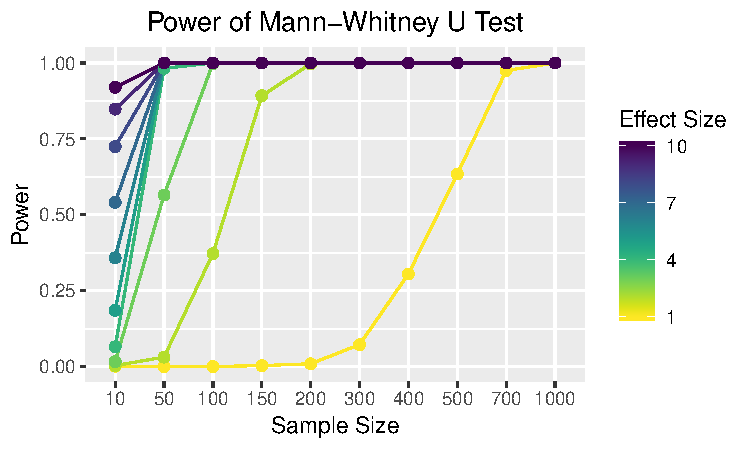
\includegraphics{../figure/power_mw.pdf}
\caption{Power of Mann-Whitney U Test under Different Scenarios}
\end{figure}

\begin{table}

\caption{\label{tab:size-tables}Size of Student's T Test}
\centering
\begin{tabular}[t]{lrrrrrrrrrr}
\toprule
\multicolumn{1}{c}{\bfseries Sample Size} & \multicolumn{5}{c}{\bfseries SD Difference} & \multicolumn{5}{c}{\bfseries SD Difference(record round to 0)} \\
\cmidrule(l{2pt}r{2pt}){1-1} \cmidrule(l{2pt}r{2pt}){2-6} \cmidrule(l{2pt}r{2pt}){7-11}
  & 0 & 3 & 5 & 8 & 10 & 0 & 3 & 5 & 8 & 10\\
\midrule
10 & 0 & 0.017 & 0.025 & 0.032 & 0.032 & 0 & 0.014 & 0.025 & 0.033 & 0.035\\
50 & 0 & 0.009 & 0.022 & 0.031 & 0.034 & 0 & 0.011 & 0.017 & 0.033 & 0.035\\
100 & 0 & 0.012 & 0.020 & 0.023 & 0.023 & 0 & 0.014 & 0.020 & 0.023 & 0.024\\
150 & 0 & 0.019 & 0.027 & 0.027 & 0.031 & 0 & 0.019 & 0.026 & 0.029 & 0.030\\
200 & 0 & 0.009 & 0.021 & 0.024 & 0.025 & 0 & 0.010 & 0.017 & 0.022 & 0.028\\
\addlinespace
300 & 0 & 0.010 & 0.022 & 0.031 & 0.034 & 0 & 0.011 & 0.025 & 0.033 & 0.036\\
400 & 0 & 0.019 & 0.029 & 0.036 & 0.038 & 0 & 0.018 & 0.030 & 0.040 & 0.041\\
500 & 0 & 0.016 & 0.025 & 0.034 & 0.039 & 0 & 0.015 & 0.025 & 0.031 & 0.038\\
700 & 0 & 0.013 & 0.022 & 0.029 & 0.034 & 0 & 0.013 & 0.020 & 0.031 & 0.033\\
1000 & 0 & 0.015 & 0.029 & 0.033 & 0.036 & 0 & 0.013 & 0.028 & 0.034 & 0.036\\
\bottomrule
\end{tabular}
\end{table}

\begin{table}

\caption{\label{tab:size-tables}Size of Mann-Whitney U Test}
\centering
\begin{tabular}[t]{lrrrrrrrrrr}
\toprule
\multicolumn{1}{c}{\bfseries Sample Size} & \multicolumn{5}{c}{\bfseries SD Difference} & \multicolumn{5}{c}{\bfseries SD Difference(record round to 0)} \\
\cmidrule(l{2pt}r{2pt}){1-1} \cmidrule(l{2pt}r{2pt}){2-6} \cmidrule(l{2pt}r{2pt}){7-11}
  & 0 & 3 & 5 & 8 & 10 & 0 & 3 & 5 & 8 & 10\\
\midrule
10 & 0 & 0.029 & 0.041 & 0.049 & 0.049 & 0 & 0.031 & 0.047 & 0.054 & 0.057\\
50 & 0 & 0.028 & 0.046 & 0.054 & 0.057 & 0 & 0.031 & 0.047 & 0.056 & 0.058\\
100 & 0 & 0.028 & 0.048 & 0.063 & 0.065 & 0 & 0.029 & 0.045 & 0.062 & 0.070\\
150 & 0 & 0.033 & 0.049 & 0.057 & 0.057 & 0 & 0.032 & 0.045 & 0.059 & 0.057\\
200 & 0 & 0.026 & 0.045 & 0.056 & 0.061 & 0 & 0.028 & 0.047 & 0.055 & 0.061\\
\addlinespace
300 & 0 & 0.036 & 0.051 & 0.066 & 0.071 & 0 & 0.034 & 0.056 & 0.067 & 0.075\\
400 & 0 & 0.043 & 0.064 & 0.074 & 0.080 & 0 & 0.044 & 0.064 & 0.076 & 0.080\\
500 & 0 & 0.034 & 0.051 & 0.064 & 0.066 & 0 & 0.027 & 0.051 & 0.063 & 0.069\\
700 & 0 & 0.029 & 0.048 & 0.054 & 0.057 & 0 & 0.034 & 0.050 & 0.058 & 0.062\\
1000 & 0 & 0.038 & 0.054 & 0.065 & 0.071 & 0 & 0.037 & 0.056 & 0.063 & 0.070\\
\bottomrule
\end{tabular}
\end{table}

\begin{figure}
\centering
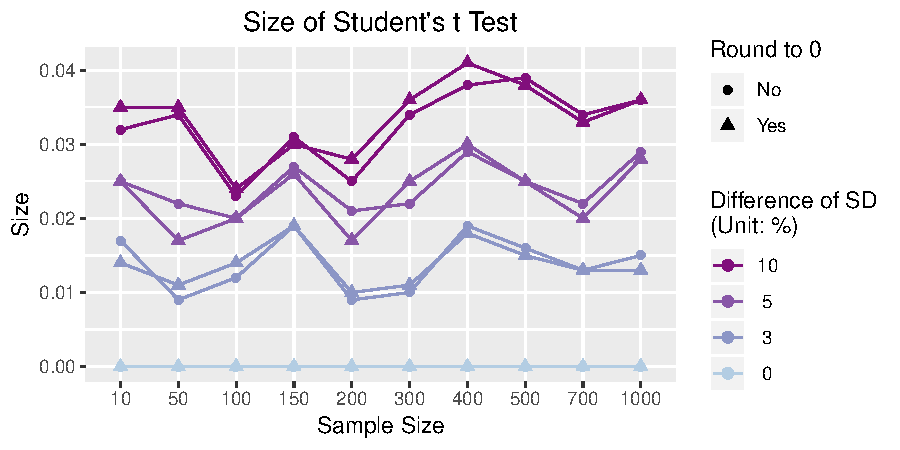
\includegraphics{../figure/size_t.pdf}
\caption{Size of Student's t Test under Different Scenarios}
\end{figure}

\begin{figure}
\centering
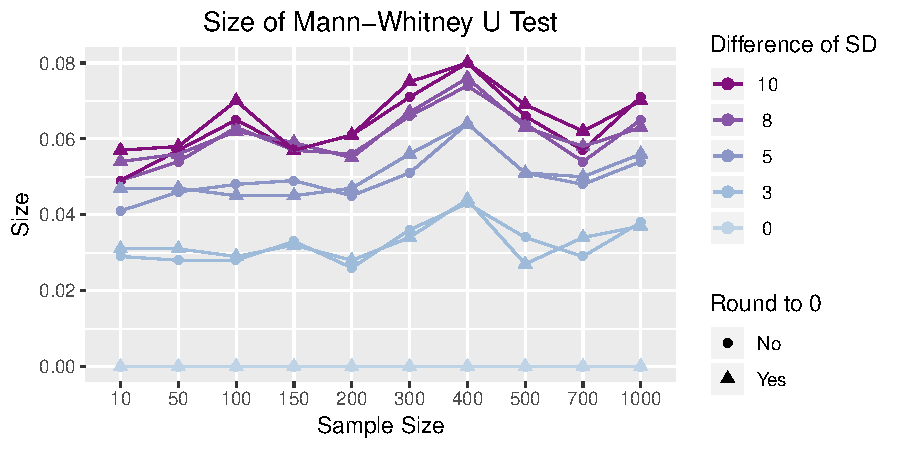
\includegraphics{../figure/size_mw.pdf}
\caption{Size of Mann-Whitney U Test under Different Scenarios}
\end{figure}

\hypertarget{conclusion}{%
\section{Conclusion}\label{conclusion}}

Here to draw conclusions! Here to draw conclusions! Here to draw
conclusions! Here to draw conclusions! Here to draw conclusions!

\newpage

\hypertarget{reference}{%
\section{Reference}\label{reference}}

\hypertarget{refs}{}
\leavevmode\hypertarget{ref-BBCNews2018}{}%
BBC News (2018) \emph{People's Vote march: Hundreds of thousands attend
London protest}. {[}Online{]}. Available from:
\url{https://www.bbc.co.uk/news/uk-45925542}.

\leavevmode\hypertarget{ref-Becker2017}{}%
Becker, S.O., Fetzer, T. \& Novy, D. (2017) Who voted for Brexit? A
comprehensive district-level analysis. \emph{Economic Policy}.
{[}Online{]} Available from:
doi:\href{https://doi.org/10.1093/epolic/eix012}{10.1093/epolic/eix012}.

\leavevmode\hypertarget{ref-ElectoralCommission2016}{}%
Electoral Commission (2016) \emph{2016 EU Referendum in the United
Kingdom}. {[}Online{]}. Available from:
\url{https://www.kaggle.com/electoralcommission/brexit-results}.

\hypertarget{appendix}{%
\section{Appendix}\label{appendix}}


\end{document}
